
\subsection{Two-dimensional Poisson Equation}

\begin{figure}[!h]
  \centering
  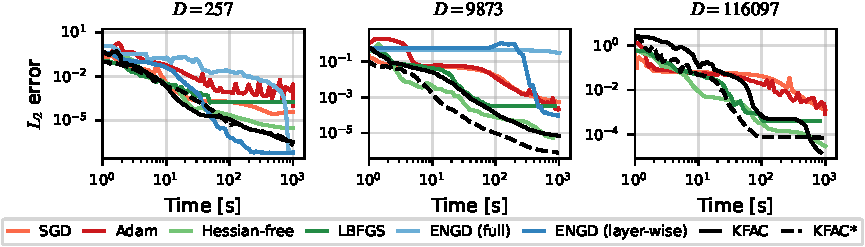
\includegraphics{../kfac_pinns_exp/exp17_groupplot_poisson2d/l2_error_over_time.pdf}
  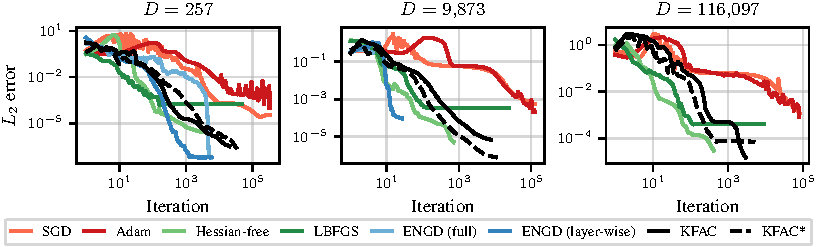
\includegraphics{../kfac_pinns_exp/exp17_groupplot_poisson2d/l2_error_over_step.pdf}
  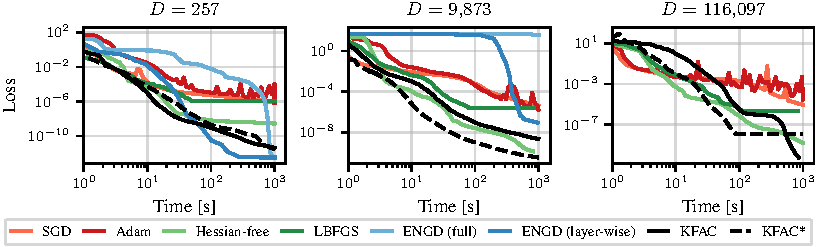
\includegraphics{../kfac_pinns_exp/exp17_groupplot_poisson2d/loss_over_time.pdf}
  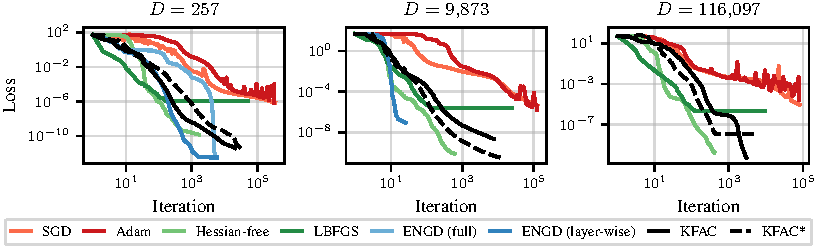
\includegraphics{../kfac_pinns_exp/exp17_groupplot_poisson2d/loss_over_step.pdf}
  \caption{$L_2$-error for learning the solution of a 2d-Poisson equation with different neural network size under a given time budget of $10^3\,\text{s}$ on an RTX 6000 GPU.}
\end{figure}

\clearpage

\subsection{Five-dimensional Poisson Equation}

\begin{figure}[!h]
  \centering
  % 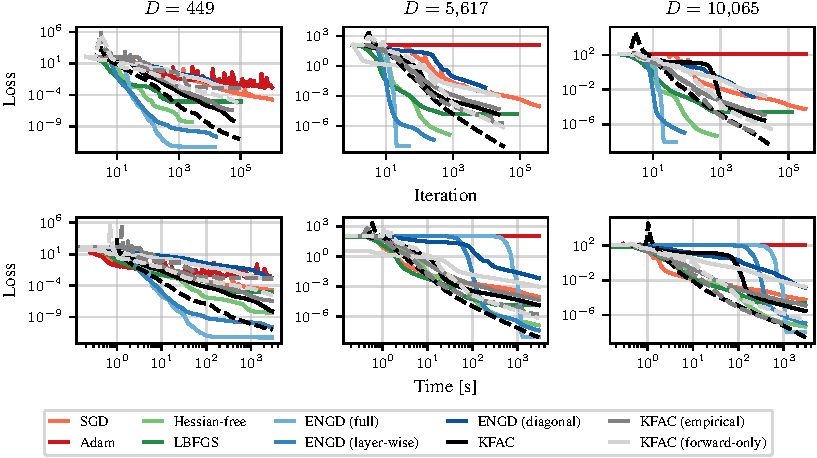
\includegraphics{../kfac_pinns_exp/exp18_groupplot_poisson5d/loss_all.pdf}
  % \\
  % 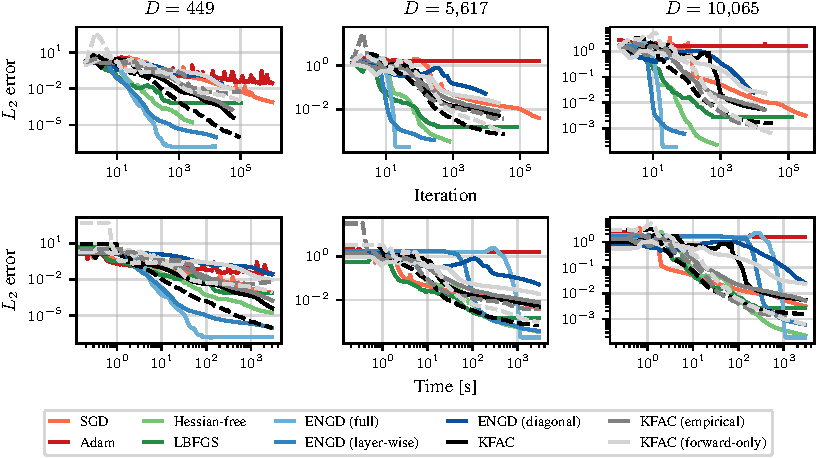
\includegraphics{../kfac_pinns_exp/exp18_groupplot_poisson5d/l2_error_all.pdf}
  \caption{Loss curves for learning the solution of a 5d-Poisson equation with different neural network size under a given time budget of $3\cdot 10^3\,\text{s}$ on an RTX 6000 GPU.
    Top row shows loss over time, bottom row shows loss over step.}
\end{figure}

%%% Local Variables:
%%% mode: latex
%%% TeX-master: "../main"
%%% End:
